% L7c lecture companion. Notebook hashes and coverage are recorded in README.md.
% Style files and Cornell seal are copied unchanged from the L7a deck (identical
% to L6c, which matches the approved L6a deck). The regression figure is the
% light PDF from ../figs/Fig-LinearRegressionModel-Schematic, copied into
% assets/ by `make figures`.
%
% Notation follows the lecture: augmented data matrix \hat{X}, augmented
% features \hat{x}_i, parameters theta, estimate \hat{theta}, and S for the
% matrix of singular values. Greek vectors (theta, epsilon) are set plain, as
% the notebook renders them and as the figure labels them.
\documentclass[aspectratio=169,11pt]{beamer}
\usepackage{vnslides}
\renewcommand{\vnlecturecode}{L7c}
\newcommand{\lecturelink}{https://github.com/varnerlab/CHEME-5800-CourseRepository-Fall-2026/blob/main/weeks/week-07/L7c/CHEME-5800-L7c-Lecture-OrdinaryLeastSquares-Fall-2026.ipynb}
\newcommand{\lablink}{https://github.com/varnerlab/CHEME-5800-CourseRepository-Fall-2026/blob/main/weeks/week-07/L7d/CHEME-5800-L7d-Lab-HousingPriceOLS-Fall-2026.ipynb}
\newcommand{\lecturesource}[1]{\note{[Sources]\par
  \href{\lecturelink}{L7c lecture: Ordinary Least Squares.}\par
  #1\par[/Sources]}}
\newcommand{\Xh}{\hat{\mathbf X}}
\newcommand{\xh}{\hat{\mathbf x}}
\newcommand{\thh}{\hat{\theta}}

\title{\texorpdfstring{{\vnheavy L7c}}{L7c}: Ordinary Least Squares}
\subtitle{\texorpdfstring{Linear models, the SVD solution, and parameter uncertainty\\[3pt]CHEME 5800 Cornell University}{Linear models, the SVD solution, and parameter uncertainty; CHEME 5800 Cornell University}}
\author{Copyright Jeffrey Varner 2026. All Rights Reserved}

\begin{document}
\special{pdf:minorversion 7}
\vntitlepage

\begin{frame}{Objectives for Today}
  How do we estimate the parameters of a linear model from data, and how
  certain are those estimates?

  \vspace{0.4em}
  {\large\textbf{\ink{Today's concepts}}}
  \vspace{0.2em}
  \begin{itemize}\setlength{\itemsep}{0.4em}
    \item \hilite{Estimate linear model parameters with ordinary least squares}:
      derive the estimate for more observations than parameters, and the
      least-norm estimate for fewer.
    \item \hilite{Compute the estimate with the singular value decomposition}:
      write it as a weighted sum of right singular vectors and compare it with
      solving the normal equations.
    \item \hilite{Quantify the uncertainty in the estimated parameters}: estimate
      the error variance, compute standard errors, and build confidence intervals.
  \end{itemize}
  \slidenote{Lecture:}{\href{\lecturelink}{Ordinary Least Squares}}
  \lecturesource{Introduction and three Learning Objectives.}
\end{frame}

\begin{frame}{Lecture and Lab}
  \textbf{\ink{Lecture:}}
  \href{\lecturelink}{Ordinary Least Squares}

  In this lecture, we derive the least-squares estimate of a linear model's
  parameters, compute it with the singular value decomposition, and quantify
  its uncertainty.

  \vspace{1.1em}
  \textbf{\ink{Lab:}}
  \href{\lablink}{L7d}

  In the lab, we build a linear model of housing prices and estimate its
  parameters with ordinary least squares.

  \vspace{0.8em}
  A linear model describes a continuous output as a weighted sum of input
  features plus a random error.
  \lecturesource{Introduction, Linear models opening sentence, and Lab section.}
\end{frame}

\begin{frame}{Observations, Model, and Residuals}
  \centering
  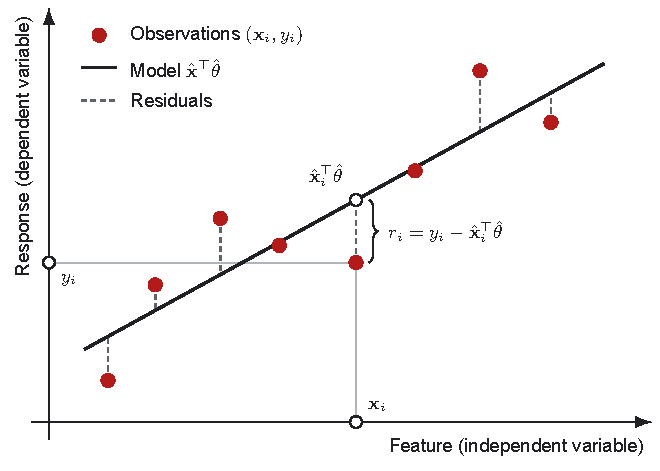
\includegraphics[width=\textwidth,height=0.63\paperheight,keepaspectratio]{assets/Fig-LinearRegressionModel-Schematic.pdf}

  \vspace{0.4em}
  \raggedright
  Each dashed segment is a \hilite{residual}. Least squares makes the sum of
  the squared residuals as small as possible.
  \lecturesource{Linear models for continuous prediction tasks: figure and caption.
    Figure: ../figs/Fig-LinearRegressionModel-Schematic (TikZ, October 5, 2026).}
\end{frame}

\begin{frame}{A Linear Model}
  Suppose a dataset $\mathcal D=\{(\mathbf x_i,y_i)\mid i=1,\ldots,n\}$ has $n$
  labeled examples, with features $\mathbf x_i\in\mathbb R^m$ and a response
  $y_i\in\mathbb R$. A \hilite{linear model} for $\mathcal D$ is:
  \[
    y_i=\xh_i^\top\theta+\epsilon_i,\qquad i=1,2,\ldots,n,
  \]
  where the augmented features $\xh_i^\top=(x_{i1},\ldots,x_{im},1)$ add a $1$
  for the intercept, $\theta\in\mathbb R^p$ with $p=m+1$ holds the unknown
  parameters, and $\epsilon_i$ is the unobserved random error. In
  matrix-vector form:
  \[
    \mathbf y=\Xh\,\theta+\epsilon,
  \]
  where the rows of $\Xh\in\mathbb R^{n\times p}$ are the $\xh_i^\top$, and
  $\mathbf y$ and $\epsilon$ stack the $y_i$ and $\epsilon_i$.

  \vspace{0.4em}
  A linear model only needs to be linear in the \hilite{parameters}:
  polynomial features such as $1,x,x^2,x^3,\ldots$ still give a linear model.
  \lecturesource{Linear models for continuous prediction tasks: index and matrix forms, and the Key insight callout.}
\end{frame}

\begin{frame}{Overdetermined Case: The Normal Equations}
  Suppose $\Xh$ is \hilite{overdetermined}, $n>p$, and the errors are
  $\epsilon\sim\mathcal N(\mathbf 0,\sigma^2\mathbf I)$ with variance $\sigma^2$.
  We minimize the sum of squared errors:
  \[
    \thh=\arg\min_{\theta}\;\tfrac12\,\|\mathbf y-\Xh\theta\|_2^2.
  \]
  Setting the gradient to zero gives the \hilite{normal equations}:
  \[
    \Xh^\top\bigl(\mathbf y-\Xh\thh\bigr)=\mathbf 0.
  \]
  The residual is orthogonal to every column of $\Xh$, so the fitted values
  $\Xh\thh$ are the \hilite{orthogonal projection} of $\mathbf y$ onto the
  column space of $\Xh$. With full column rank, $r(\Xh)=p$:
  \[
    \thh=\bigl(\Xh^\top\Xh\bigr)^{-1}\Xh^\top\mathbf y.
  \]
  \lecturesource{Ordinary least squares: Overdetermined data matrix, objective, normal equations, projection, and solution.}
\end{frame}

\begin{frame}{The OLS Estimate Is Unbiased}
  Substituting the model $\mathbf y=\Xh\theta+\epsilon$ into the solution:
  \[
    \thh=\bigl(\Xh^\top\Xh\bigr)^{-1}\Xh^\top\bigl(\Xh\theta+\epsilon\bigr)
       =\theta+\bigl(\Xh^\top\Xh\bigr)^{-1}\Xh^\top\epsilon.
  \]
  \begin{itemize}\setlength{\itemsep}{0.6em}
    \item \hilite{Unbiased estimator}: the errors have mean zero, so
      $\mathbb E[\thh]=\theta$. On average, we get the right answer.
    \item \hilite{Parameter uncertainty}: because $\epsilon$ is random, $\thh$ is
      a random vector with its own distribution. We quantify it with standard
      errors and confidence intervals.
    \item \hilite{Bayesian connection}: Bayesian linear regression goes one step
      further and treats the parameters themselves as random variables.
  \end{itemize}
  \lecturesource{Ordinary least squares: Overdetermined data matrix, decomposition and Key insights.}
\end{frame}

\begin{frame}{Underdetermined Case: Least-Norm Solution}
  Suppose $\Xh$ is \hilite{underdetermined}, $n<p$, with full row rank,
  $r(\Xh)=n$. Infinitely many parameter vectors satisfy $\Xh\theta=\mathbf y$
  exactly, and we choose the smallest:
  \[
    \min_{\theta}\;\|\theta\|_2^2\quad\text{subject to}\quad\Xh\theta=\mathbf y.
  \]
  Because $\Xh\Xh^\top$ is invertible, the least-norm solution is:
  \[
    \thh=\Xh^\top\bigl(\Xh\Xh^\top\bigr)^{-1}\mathbf y
       =\mathbf P\,\theta+\Xh^\top\bigl(\Xh\Xh^\top\bigr)^{-1}\epsilon,
    \qquad
    \mathbf P=\Xh^\top\bigl(\Xh\Xh^\top\bigr)^{-1}\Xh.
  \]
  The matrix $\mathbf P$ is the orthogonal projection onto the row space of
  $\Xh$. Since $\mathbb E[\thh]=\mathbf P\theta$, the estimate is
  \hilite{biased} unless $\theta$ already lies in that subspace.
  \lecturesource{Ordinary least squares: Underdetermined data matrix and the Projection interpretation callout.}
\end{frame}

\begin{frame}{Why Choose the Smallest Solution?}
  Every exact solution is the least-norm solution $\thh$ plus a vector
  $\mathbf z$ in the \hilite{null space} of $\Xh$, so $\Xh\mathbf z=\mathbf 0$.
  The least-norm solution lies in the row space, which is orthogonal to the
  null space:
  \[
    \|\thh+\mathbf z\|_2^2=\|\thh\|_2^2+\|\mathbf z\|_2^2.
  \]
  Adding $\mathbf z$ makes the parameter vector longer without changing the
  predictions at the observed data. The least-norm solution keeps only the
  part of $\theta$ that the data determine.

  \vspace{0.6em}
  \hilite{Regularization} adds a penalty to the loss function to prevent
  overfitting; Ridge (L2) and Lasso (L1) are common choices. The least-norm
  solution has the same preference for small parameters as L2 regularization.
  \lecturesource{Ordinary least squares: Underdetermined data matrix, Important questions.}
\end{frame}

\begin{frame}{SVD Solution of the Least-Squares Problem}
  The SVD of the data matrix is $\Xh=\mathbf U\mathbf S\mathbf V^\top$, with
  orthogonal $\mathbf U\in\mathbb R^{n\times n}$ and
  $\mathbf V\in\mathbb R^{p\times p}$, and the singular values
  $\sigma_1\ge\cdots\ge\sigma_r>0$, $r=r(\Xh)$, on the diagonal of
  $\mathbf S\in\mathbb R^{n\times p}$. The least-squares estimate is:
  \[
    \thh=\mathbf V\,\mathbf S^\dagger\,\mathbf U^\top\mathbf y
    \quad\Longrightarrow\quad
    \boxed{\thh=\sum_{i=1}^{r(\Xh)}\left(\frac{\mathbf u_i^\top\mathbf y}{\sigma_i}\right)\mathbf v_i}
  \]
  where the Moore--Penrose pseudoinverse $\mathbf S^\dagger\in\mathbb R^{p\times n}$
  transposes $\mathbf S$ and replaces each nonzero $\sigma_i$ with $1/\sigma_i$,
  and $\mathbf u_i$ and $\mathbf v_i$ are the columns of $\mathbf U$ and $\mathbf V$.

  \vspace{0.5em}
  The same formula gives the OLS estimate under full column rank and the
  least-norm estimate under full row rank.
  \lecturesource{SVD solution of the least-squares problem: factorization, pseudoinverse, and boxed sum.}
\end{frame}

\begin{frame}{Reading the SVD Solution}
  The estimate is a weighted sum of the right singular vectors $\mathbf v_i$.
  Each weight is the dot product $\mathbf u_i^\top\mathbf y$ divided by the
  singular value $\sigma_i$.

  \vspace{0.6em}
  \begin{itemize}\setlength{\itemsep}{0.8em}
    \item \hilite{Mode contribution}: each term projects $\mathbf y$ onto the
      data-space direction $\mathbf u_i$ and maps the result onto the
      parameter-space direction $\mathbf v_i$.
    \item \hilite{Noise amplification}: when $\sigma_i$ is small, the factor
      $1/\sigma_i$ magnifies measurement errors in $\mathbf y$ along
      $\mathbf v_i$. This identifies unreliable components of the solution and
      motivates regularization that dampens the contributions of small singular values.
  \end{itemize}
  \lecturesource{SVD solution of the least-squares problem: weighted-sum reading and Key insights.}
\end{frame}

\begin{frame}{SVD versus Direct Methods}
  \begin{itemize}\setlength{\itemsep}{0.7em}
    \item \hilite{Rank-deficient matrices}: without full column rank,
      $\Xh^\top\Xh$ is singular. The SVD skips the zero singular values and
      returns the minimum-norm least-squares solution.
    \item \hilite{Ill-conditioned problems}: the condition number $\kappa$ is the
      ratio of the largest to the smallest singular value. With full column
      rank, $\kappa(\Xh^\top\Xh)=\kappa(\Xh)^2$, so forming $\Xh^\top\Xh$
      squares it; the SVD factors $\Xh$ directly.
    \item \hilite{Cost}: the thin SVD costs $O(\min(np^2,n^2p))$; the direct
      method costs $O(np^2)$ to form $\Xh^\top\Xh$ and $O(p^3)$ to solve. For
      $n\gg p$, both scale as $O(np^2)$, and the direct method is often faster.
  \end{itemize}

  \vspace{0.6em}
  For a rectangular matrix \texttt{X}, Julia's backslash operator,
  \texttt{X \textbackslash{} y}, solves least squares from a pivoted QR
  factorization of \texttt{X} and never forms \texttt{X' * X}.
  \lecturesource{SVD solution of the least-squares problem: SVD versus direct methods, computational trade-offs, and the backslash operator.}
\end{frame}

\begin{frame}{The Error Model}
  We assume $\epsilon\sim\mathcal N(\mathbf 0,\sigma^2\mathbf I)$: each error
  is independent and normal, with mean zero and constant variance $\sigma^2$.

  \vspace{0.4em}
  \begin{itemize}\setlength{\itemsep}{0.55em}
    \item \hilite{Normality} gives the estimates exact distributions, for
      confidence intervals and hypothesis tests. With zero-mean, uncorrelated,
      constant-variance errors, OLS is the best linear unbiased estimator (BLUE).
    \item \hilite{Uncorrelated errors}: $\sigma^2\mathbf I$ is diagonal, so
      $\mathrm{Cov}(\epsilon_i,\epsilon_j)=0$ for $i\ne j$. The parameter
      variance relies on this structure.
    \item \hilite{Reality check}: by the Central Limit Theorem, the estimates are
      often approximately normal for large samples, even when the errors are not.
  \end{itemize}

  \vspace{0.4em}
  From here on, $\Xh$ is overdetermined with full column rank, and we treat it
  as fixed, so all of the randomness in $\thh$ comes from $\epsilon$.
  \lecturesource{Understanding the error model: assumption, Normality and Uncorrelated errors callouts, Reality check, and scope.}
\end{frame}

\begin{frame}{Estimating the Error Variance}
  Since the true variance $\sigma^2$ is unknown, we estimate it from the
  residuals $\mathbf r=\mathbf y-\Xh\thh$:
  \[
    \hat\sigma^2=\frac{\|\mathbf r\|_2^2}{n-p}=\frac{1}{n-p}\sum_{i=1}^{n}r_i^2,
    \qquad r_i=y_i-\xh_i^\top\thh.
  \]

  \vspace{0.4em}
  Dividing by $n-p$ accounts for the degrees of freedom used up by estimating
  $p$ parameters, which makes $\hat\sigma^2$ an \hilite{unbiased} estimator of
  $\sigma^2$.

  \vspace{0.6em}
  This is why we need $n>p$: with full row rank and $n\le p$, the fit passes
  through every observation, so the residuals are zero and carry no
  information about $\sigma^2$.
  \lecturesource{Understanding the error model: Estimating the error variance and its Key insight.}
\end{frame}

\begin{frame}{Parameter Uncertainty}
  Since $\thh=\theta+(\Xh^\top\Xh)^{-1}\Xh^\top\epsilon$ and $\theta$ is
  constant, we use $\mathrm{Var}(\mathbf A\mathbf z)=\mathbf A\,\mathrm{Var}(\mathbf z)\,\mathbf A^\top$
  for a constant matrix $\mathbf A$ and a random vector $\mathbf z$, with
  $\mathrm{Var}(\epsilon)=\sigma^2\mathbf I$:
  \[
    \mathrm{Var}(\thh)
    =\bigl(\Xh^\top\Xh\bigr)^{-1}\Xh^\top\bigl(\sigma^2\mathbf I\bigr)\Xh\bigl(\Xh^\top\Xh\bigr)^{-1}
    =\sigma^2\bigl(\Xh^\top\Xh\bigr)^{-1}.
  \]
  The \hilite{standard error} of $\thh_j$ is its estimated standard deviation,
  with the unknown $\sigma^2$ replaced by $\hat\sigma^2$:
  \[
    \mathrm{SE}(\thh_j)=\sqrt{\hat\sigma^2\,\bigl[(\Xh^\top\Xh)^{-1}\bigr]_{jj}}.
  \]
  \lecturesource{Understanding the error model: Parameter uncertainty derivation and the standard error.}
\end{frame}

\begin{frame}{What Standard Errors Give Us}
  \begin{itemize}\setlength{\itemsep}{0.9em}
    \item \hilite{Confidence intervals}: for large samples,
      $\thh_j\pm1.96\,\mathrm{SE}(\thh_j)$ is an approximate 95\% confidence
      interval for $\theta_j$. For finite samples, we use the t-distribution.
    \item \hilite{Hypothesis tests}: to test whether $\theta_j=0$, compare
      $t_j=\thh_j/\mathrm{SE}(\thh_j)$ with a t-distribution with $n-p$ degrees
      of freedom. The p-value is the probability of a value at least this
      extreme if $\theta_j$ is actually $0$.
    \item \hilite{Prediction intervals}: the margin around a new prediction
      combines the parameter covariance $\hat\sigma^2(\Xh^\top\Xh)^{-1}$ with
      the error variance $\hat\sigma^2$ of the new observation.
  \end{itemize}
  \lecturesource{Understanding the error model: Standard errors are essential for callout.}
\end{frame}

\begin{frame}{Confidence Intervals}
  A 95\% confidence interval contains the true $\theta_j$ in about 95\% of
  repeated experiments. Under the normal, constant-variance error model:
  \[
    T_j=\frac{\thh_j-\theta_j}{\mathrm{SE}(\thh_j)}\sim t_\nu,\qquad\nu=n-p.
  \]
  Let $c=t_{1-\alpha/2,\nu}$, the $(1-\alpha/2)$ quantile of the
  t-distribution, where $\alpha$ is the significance level ($\alpha=0.05$ for
  95\%). Inverting $\Pr(-c\le T_j\le c)=1-\alpha$ bounds $\theta_j$:
  \[
    \boxed{\thh_j\pm t_{1-\alpha/2,\nu}\,\hat\sigma\sqrt{\bigl[(\Xh^\top\Xh)^{-1}\bigr]_{jj}}}
  \]
  One-sided intervals follow the same way from one tail.
  \lecturesource{Understanding the error model: A note about confidence intervals.}
\end{frame}

\begin{frame}{Summary}
  We estimated the parameters of a linear model with least squares, computed
  the estimate with the SVD, and quantified its uncertainty.

  \vspace{0.6em}
  {\large\textbf{\ink{Key takeaways}}}
  \vspace{0.3em}
  \begin{itemize}\setlength{\itemsep}{0.9em}
    \item \textbf{\ink{Overdetermined and underdetermined problems.}} OLS projects
      the data onto the column space; with too few observations, we take the least-norm solution.
    \item \textbf{\ink{Least squares with the SVD.}} The estimate is a weighted sum
      of right singular vectors, and small singular values amplify noise.
    \item \textbf{\ink{Parameter uncertainty.}} The residuals give the error
      variance, which gives standard errors and confidence intervals.
  \end{itemize}

  \vspace{0.8em}
  In the L7d lab, we fit a linear model of housing prices.
  \lecturesource{Summary: three key takeaways and concluding sentence.}
\end{frame}

\end{document}
